\section{Depth and Regime Transition}
\label{sec:regime}

The closed-form decomposition of Section~\ref{sec:method} makes a
falsifiable prediction about where, in depth and scale, the key-cosine law
should hold and where it should break down. We test it directly: we trace the
within-probe coupling across the editable layer range of Llama-3.2-1B,
identify the depth at which a second geometric quantity overtakes key-cosine
as the dominant predictor, and show that the same transition recurs, in sign,
as a function of the model's overall damage regime rather than depth alone.

\subsection{The within-probe layer law}
Fixing a probe, damage ranks across edits by $S\cdot|C|$; when $S$ has
limited spread relative to $C$, the within-probe Spearman correlation down
that probe's column is high. Across 3 seeds on the saved gate matrices, the
clean key-cosine metric traces an inverted-U in depth: $\rho =
\gWithinLeight{}\rightarrow\gWithinLten{}\rightarrow\gWithinLtwelve{}$
(peak, L12) $\rightarrow\gWithinLfourteen{}$ (L14), with
$\text{frac\_positive}=1.0$ and permutation-$p$ at the \gPermFloor{} floor at
every layer (Figure~\ref{fig:layerlaw}(a)). The rise from L8 to L12 and the
fall by L14 are not an artifact of a shrinking sample: every layer uses the
identical known-fact and successful-edit filters, probe bank, and within-probe
partialling procedure of Section~\ref{sec:gate}, so the curve reflects a
genuine property of how the edited layer's key geometry relates to collateral
damage as depth increases.

\subsection{The L14 crossover}
The rank of damage down a column is governed by the relative spread of $S$
versus $|C|$ at that layer. Mid-layer, $|C|$ carries most of the cross-edit
variance and geometry dominates the ranking; at L14, $|C|$ saturates (mean
$|C|$ rises to \meanCLfourteen{} versus \meanCbandLo{}--\meanCbandHi{}
across the L8--L12 band) while $S$ becomes the dominant varying factor, so
matrix-norm-growth overtakes key-cosine as the within-probe predictor.
Head-to-head, the true norm-growth$\rightarrow$damage within-probe $\rho$ is
\ngWithinLeight{} / \ngWithinLten{} / \ngWithinLtwelve{} /
\ngWithinLfourteen{} at L8/L10/L12/L14: key-cosine wins at L8, L10, and L12,
and norm-growth overtakes at L14
($\ngWithinLfourteen{} > \gWithinLfourteen{}$), on all 3 seeds
(Figure~\ref{fig:layerlaw}(a)). This crossover survives the same
confound-clean controls as the headline law -- double-centering and
norm-growth partialling -- so it is a genuine depth effect on the
confound-clean metric, not a flat-statistics artifact of comparing two
quantities with different variance structure.

\subsection{The scale/regime law}
The transition is not merely a depth effect but a \emph{damage-regime}
effect: the \emph{sign} of the coupling tracks the sign of the
\emph{mean damage}, not the layer index by itself. At Llama-3B L24, a
positive-damage regime, the within-probe $\rho = \regimeThreeB{}$ (3-seed
range \regimeThreeBLo{}--\regimeThreeBHi{}); at Llama-8B L24, a
net-improvement regime in which the mean per-edit damage is negative, the
coupling is $\rho = \regimeEightB{}$ (3-seed mean, per-seed range
\regimeEightBHi{} to \regimeEightBLo{}). Within the 8B model the sign itself
flips with depth: L24 gives \regimeEightB{} (3-seed) while L16 gives
$+\regimeEightBLsixteen{}$ and L28 gives $+\regimeEightBLtwentyeight{}$
(single seed) -- so the same architecture, edited with the same recipe, can
sit on either side of the sign flip depending on which layer is edited and
which damage regime that layer falls into (Figure~\ref{fig:layerlaw}(b)).
The norm-growth transition itself tracks \emph{relative}, not absolute,
depth: 8B L28 sits at \relDepthEightBLtwentyeight{} relative depth -- the
same relative position as 1B's L14 -- and shows the norm-growth dominance
directionally, though attenuated by roughly \ngAttenPct\% relative to the 1B
model. Taken together, the settled claim is that the sign of the
coupling tracks the sign of the damage regime, on both sides, across 3-seed
evidence, while the magnitude of that coupling is attenuated at the largest
scale tested ($|\rho|\approx\regimeMagAttenLo{}$--$\regimeMagAttenHi{}$ at 8B,
versus $0.38$ at 3B). Its generalization across
architecture families beyond Llama, in both sign and unsigned magnitude, is
reported in Figure~\ref{fig:crossarch} and the architecture arm of
Section~\ref{sec:dissociation}.

% =====================================================================
% fig:layerlaw (IEEE de-merge, part 1 of former figA_lawtransfer / F1+F7).
% Layer-law panels only: (a) depth, (b) regime-across-scale. The
% architecture-generalization panels move to the companion single-column
% figure fig:crossarch (figA2_crossarch.tex), referenced from
% Section~\ref{sec:dissociation}.
% Body ported from the R/tikzDevice pipeline (figures/figA1.tex, IEEE
% dimensions) rather than hand-authored pgfplots, for consistency with the
% rest of the figure set. Same source JSONs, no new numbers.
% Regenerate: Rscript figures/make_figures_ieee.R
% =====================================================================
\begin{figure*}[t]
\centering
% =====================================================================
% figA1  — R/ggplot2 -> tikzDevice (parallel to ../figures-tex/figA1_layerlaw.tex)
% Canonical-JSON-only. Regenerate: Rscript figures/make_figures_ieee.R
% Provenance (JSON path :: field = plotted value), one line per series:
% SOURCE: results/G1_L8_analysis.json :: aggregate.within_probe_mean_across_seeds = 0.3951
% SOURCE: results/G1_L8_analysis.json :: mean(per_seed[].within_probe_mean_normgrowth) = 0.0825
% SOURCE: results/G1_L10_analysis.json :: aggregate.within_probe_mean_across_seeds = 0.5337
% SOURCE: results/G1_L10_analysis.json :: mean(per_seed[].within_probe_mean_normgrowth) = 0.2458
% SOURCE: results/G1_L12_analysis.json :: aggregate.within_probe_mean_across_seeds = 0.6018
% SOURCE: results/G1_L12_analysis.json :: mean(per_seed[].within_probe_mean_normgrowth) = 0.5087
% SOURCE: results/G1_L14_analysis.json :: aggregate.within_probe_mean_across_seeds = 0.3006
% SOURCE: results/G1_L14_analysis.json :: mean(per_seed[].within_probe_mean_normgrowth) = 0.5019
% SOURCE: results/C3_regime_3b_L24_r4.json :: aggregate.within_probe_mean_across_seeds = 0.3764
% SOURCE: results/C3_llama8b_r3.json :: per_seed[L16].within_probe_mean = 0.1734
% SOURCE: results/C3_llama8b_r3.json :: per_seed[L24].within_probe_mean = -0.1169
% SOURCE: results/C3_llama8b_r3.json :: per_seed[L28].within_probe_mean = 0.1554
% =====================================================================
% !TEX encoding = UTF-8 Unicode
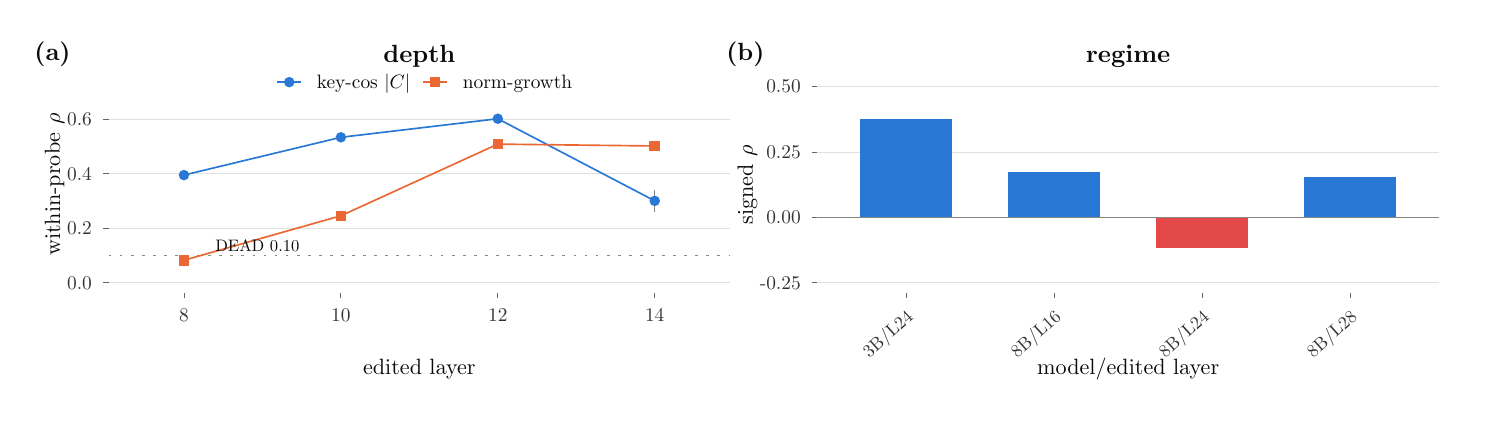
\begin{tikzpicture}[x=1pt,y=1pt]
\definecolor{fillColor}{RGB}{255,255,255}
\path[use as bounding box,fill=fillColor,fill opacity=0.00] (0,0) rectangle (517.45,133.70);
\begin{scope}
\path[clip] (  0.00,  0.00) rectangle (517.45,133.70);
\definecolor{drawColor}{RGB}{255,255,255}
\definecolor{fillColor}{RGB}{255,255,255}

\path[draw=drawColor,line width= 0.6pt,line join=round,line cap=round,fill=fillColor] ( -0.00,  0.00) rectangle (517.45,133.70);
\end{scope}
\begin{scope}
\path[clip] (  5.50,  5.50) rectangle (255.81,128.20);
\definecolor{fillColor}{RGB}{255,255,255}

\path[fill=fillColor] (  5.50,  5.50) rectangle (255.81,128.20);
\end{scope}
\begin{scope}
\path[clip] (255.81,  5.50) rectangle (511.95,128.20);
\definecolor{fillColor}{RGB}{255,255,255}

\path[fill=fillColor] (255.81,  5.50) rectangle (511.95,128.20);
\end{scope}
\begin{scope}
\path[clip] ( 29.24, 37.97) rectangle (253.81,115.98);
\definecolor{drawColor}{RGB}{225,224,217}

\path[draw=drawColor,line width= 0.3pt,line join=round] ( 29.24, 41.52) --
	(253.81, 41.52);

\path[draw=drawColor,line width= 0.3pt,line join=round] ( 29.24, 61.22) --
	(253.81, 61.22);

\path[draw=drawColor,line width= 0.3pt,line join=round] ( 29.24, 80.91) --
	(253.81, 80.91);

\path[draw=drawColor,line width= 0.3pt,line join=round] ( 29.24,100.61) --
	(253.81,100.61);
\definecolor{drawColor}{RGB}{137,135,129}

\path[draw=drawColor,line width= 0.3pt,dash pattern=on 1pt off 3pt ,line join=round] ( 29.24, 51.37) -- (253.81, 51.37);

\path[draw=drawColor,line width= 0.4pt,line join=round] ( 56.46, 81.48) --
	( 56.46, 81.48);

\path[draw=drawColor,line width= 0.4pt,line join=round] ( 56.46, 81.48) --
	( 56.46, 79.39);

\path[draw=drawColor,line width= 0.4pt,line join=round] ( 56.46, 79.39) --
	( 56.46, 79.39);

\path[draw=drawColor,line width= 0.4pt,line join=round] (113.17, 95.12) --
	(113.17, 95.12);

\path[draw=drawColor,line width= 0.4pt,line join=round] (113.17, 95.12) --
	(113.17, 93.05);

\path[draw=drawColor,line width= 0.4pt,line join=round] (113.17, 93.05) --
	(113.17, 93.05);

\path[draw=drawColor,line width= 0.4pt,line join=round] (169.88,102.65) --
	(169.88,102.65);

\path[draw=drawColor,line width= 0.4pt,line join=round] (169.88,102.65) --
	(169.88, 98.93);

\path[draw=drawColor,line width= 0.4pt,line join=round] (169.88, 98.93) --
	(169.88, 98.93);

\path[draw=drawColor,line width= 0.4pt,line join=round] (226.59, 75.09) --
	(226.59, 75.09);

\path[draw=drawColor,line width= 0.4pt,line join=round] (226.59, 75.09) --
	(226.59, 67.15);

\path[draw=drawColor,line width= 0.4pt,line join=round] (226.59, 67.15) --
	(226.59, 67.15);
\definecolor{drawColor}{RGB}{42,120,214}

\path[draw=drawColor,line width= 0.6pt,line join=round] ( 56.46, 80.43) --
	(113.17, 94.08) --
	(169.88,100.79) --
	(226.59, 71.12);
\definecolor{drawColor}{RGB}{235,104,52}

\path[draw=drawColor,line width= 0.6pt,line join=round] ( 56.46, 49.65) --
	(113.17, 65.73) --
	(169.88, 91.62) --
	(226.59, 90.95);
\definecolor{fillColor}{RGB}{42,120,214}

\path[fill=fillColor] ( 56.46, 80.43) circle (  1.90);

\path[fill=fillColor] (113.17, 94.08) circle (  1.90);

\path[fill=fillColor] (169.88,100.79) circle (  1.90);

\path[fill=fillColor] (226.59, 71.12) circle (  1.90);
\definecolor{fillColor}{RGB}{235,104,52}

\path[fill=fillColor] ( 54.56, 47.75) --
	( 58.36, 47.75) --
	( 58.36, 51.54) --
	( 54.56, 51.54) --
	cycle;

\path[fill=fillColor] (111.27, 63.83) --
	(115.07, 63.83) --
	(115.07, 67.63) --
	(111.27, 67.63) --
	cycle;

\path[fill=fillColor] (167.98, 89.73) --
	(171.78, 89.73) --
	(171.78, 93.52) --
	(167.98, 93.52) --
	cycle;

\path[fill=fillColor] (224.69, 89.05) --
	(228.49, 89.05) --
	(228.49, 92.84) --
	(224.69, 92.84) --
	cycle;
\definecolor{drawColor}{RGB}{11,11,11}

\node[text=drawColor,anchor=base west,inner sep=0pt, outer sep=0pt, scale=  0.60] at ( 67.80, 52.87) {DEAD 0.10};
\end{scope}
\begin{scope}
\path[clip] (  0.00,  0.00) rectangle (517.45,133.70);
\definecolor{drawColor}{gray}{0.20}

\node[text=drawColor,anchor=base east,inner sep=0pt, outer sep=0pt, scale=  0.70] at ( 23.19, 39.24) {0.0};

\node[text=drawColor,anchor=base east,inner sep=0pt, outer sep=0pt, scale=  0.70] at ( 23.19, 58.94) {0.2};

\node[text=drawColor,anchor=base east,inner sep=0pt, outer sep=0pt, scale=  0.70] at ( 23.19, 78.64) {0.4};

\node[text=drawColor,anchor=base east,inner sep=0pt, outer sep=0pt, scale=  0.70] at ( 23.19, 98.33) {0.6};
\end{scope}
\begin{scope}
\path[clip] (  0.00,  0.00) rectangle (517.45,133.70);
\definecolor{drawColor}{gray}{0.40}

\path[draw=drawColor,line width= 0.3pt,line join=round] ( 27.24, 41.52) --
	( 29.24, 41.52);

\path[draw=drawColor,line width= 0.3pt,line join=round] ( 27.24, 61.22) --
	( 29.24, 61.22);

\path[draw=drawColor,line width= 0.3pt,line join=round] ( 27.24, 80.91) --
	( 29.24, 80.91);

\path[draw=drawColor,line width= 0.3pt,line join=round] ( 27.24,100.61) --
	( 29.24,100.61);
\end{scope}
\begin{scope}
\path[clip] (  0.00,  0.00) rectangle (517.45,133.70);
\definecolor{drawColor}{gray}{0.40}

\path[draw=drawColor,line width= 0.3pt,line join=round] ( 56.46, 35.97) --
	( 56.46, 37.97);

\path[draw=drawColor,line width= 0.3pt,line join=round] (113.17, 35.97) --
	(113.17, 37.97);

\path[draw=drawColor,line width= 0.3pt,line join=round] (169.88, 35.97) --
	(169.88, 37.97);

\path[draw=drawColor,line width= 0.3pt,line join=round] (226.59, 35.97) --
	(226.59, 37.97);
\end{scope}
\begin{scope}
\path[clip] (  0.00,  0.00) rectangle (517.45,133.70);
\definecolor{drawColor}{gray}{0.20}

\node[text=drawColor,anchor=base,inner sep=0pt, outer sep=0pt, scale=  0.70] at ( 56.46, 27.36) {8};

\node[text=drawColor,anchor=base,inner sep=0pt, outer sep=0pt, scale=  0.70] at (113.17, 27.36) {10};

\node[text=drawColor,anchor=base,inner sep=0pt, outer sep=0pt, scale=  0.70] at (169.88, 27.36) {12};

\node[text=drawColor,anchor=base,inner sep=0pt, outer sep=0pt, scale=  0.70] at (226.59, 27.36) {14};
\end{scope}
\begin{scope}
\path[clip] (  0.00,  0.00) rectangle (517.45,133.70);
\definecolor{drawColor}{RGB}{11,11,11}

\node[text=drawColor,anchor=base,inner sep=0pt, outer sep=0pt, scale=  0.80] at (141.53,  8.23) {edited layer};
\end{scope}
\begin{scope}
\path[clip] (  0.00,  0.00) rectangle (517.45,133.70);
\definecolor{drawColor}{RGB}{11,11,11}

\node[text=drawColor,rotate= 90.00,anchor=base,inner sep=0pt, outer sep=0pt, scale=  0.80] at ( 11.71, 76.97) {within-probe $\rho$};
\end{scope}
\begin{scope}
\path[clip] (  0.00,  0.00) rectangle (517.45,133.70);
\definecolor{drawColor}{RGB}{42,120,214}

\path[draw=drawColor,line width= 0.6pt,line join=round] ( 90.12,114.01) -- ( 98.92,114.01);
\definecolor{fillColor}{RGB}{42,120,214}

\path[fill=fillColor] ( 94.52,114.01) circle (  1.90);
\end{scope}
\begin{scope}
\path[clip] (  0.00,  0.00) rectangle (517.45,133.70);
\definecolor{drawColor}{RGB}{235,104,52}

\path[draw=drawColor,line width= 0.6pt,line join=round] (142.86,114.01) -- (151.66,114.01);
\definecolor{fillColor}{RGB}{235,104,52}

\path[fill=fillColor] (145.36,112.12) --
	(149.16,112.12) --
	(149.16,115.91) --
	(145.36,115.91) --
	cycle;
\end{scope}
\begin{scope}
\path[clip] (  0.00,  0.00) rectangle (517.45,133.70);
\definecolor{drawColor}{RGB}{11,11,11}

\node[text=drawColor,anchor=base west,inner sep=0pt, outer sep=0pt, scale=  0.70] at (104.52,111.74) {key-cos $|C|$};
\end{scope}
\begin{scope}
\path[clip] (  0.00,  0.00) rectangle (517.45,133.70);
\definecolor{drawColor}{RGB}{11,11,11}

\node[text=drawColor,anchor=base west,inner sep=0pt, outer sep=0pt, scale=  0.70] at (157.26,111.74) {norm-growth};
\end{scope}
\begin{scope}
\path[clip] (  0.00,  0.00) rectangle (517.45,133.70);
\definecolor{drawColor}{RGB}{11,11,11}

\node[text=drawColor,anchor=base,inner sep=0pt, outer sep=0pt, scale=  0.90] at (141.53,121.00) {\bfseries depth};
\end{scope}
\begin{scope}
\path[clip] (  0.00,  0.00) rectangle (517.45,133.70);
\definecolor{drawColor}{RGB}{11,11,11}

\node[text=drawColor,anchor=base,inner sep=0pt, outer sep=0pt, scale=  0.90] at (  8.97,121.69) {\bfseries (a)};
\end{scope}
\begin{scope}
\path[clip] (285.38, 37.97) rectangle (509.95,115.98);
\definecolor{drawColor}{RGB}{225,224,217}

\path[draw=drawColor,line width= 0.3pt,line join=round] (285.38, 41.52) --
	(509.95, 41.52);

\path[draw=drawColor,line width= 0.3pt,line join=round] (285.38, 65.16) --
	(509.95, 65.16);

\path[draw=drawColor,line width= 0.3pt,line join=round] (285.38, 88.79) --
	(509.95, 88.79);

\path[draw=drawColor,line width= 0.3pt,line join=round] (285.38,112.43) --
	(509.95,112.43);
\definecolor{fillColor}{RGB}{42,120,214}

\path[fill=fillColor] (300.89, 65.16) rectangle (334.04,100.75);

\path[fill=fillColor] (354.36, 65.16) rectangle (387.51, 81.55);
\definecolor{fillColor}{RGB}{227,73,72}

\path[fill=fillColor] (407.83, 54.10) rectangle (440.98, 65.16);
\definecolor{fillColor}{RGB}{42,120,214}

\path[fill=fillColor] (461.30, 65.16) rectangle (494.45, 79.85);
\definecolor{drawColor}{RGB}{137,135,129}

\path[draw=drawColor,line width= 0.3pt,line join=round] (285.38, 65.16) -- (509.95, 65.16);
\end{scope}
\begin{scope}
\path[clip] (  0.00,  0.00) rectangle (517.45,133.70);
\definecolor{drawColor}{gray}{0.20}

\node[text=drawColor,anchor=base east,inner sep=0pt, outer sep=0pt, scale=  0.70] at (279.33, 39.24) {-0.25};

\node[text=drawColor,anchor=base east,inner sep=0pt, outer sep=0pt, scale=  0.70] at (279.33, 62.88) {0.00};

\node[text=drawColor,anchor=base east,inner sep=0pt, outer sep=0pt, scale=  0.70] at (279.33, 86.52) {0.25};

\node[text=drawColor,anchor=base east,inner sep=0pt, outer sep=0pt, scale=  0.70] at (279.33,110.15) {0.50};
\end{scope}
\begin{scope}
\path[clip] (  0.00,  0.00) rectangle (517.45,133.70);
\definecolor{drawColor}{gray}{0.40}

\path[draw=drawColor,line width= 0.3pt,line join=round] (283.38, 41.52) --
	(285.38, 41.52);

\path[draw=drawColor,line width= 0.3pt,line join=round] (283.38, 65.16) --
	(285.38, 65.16);

\path[draw=drawColor,line width= 0.3pt,line join=round] (283.38, 88.79) --
	(285.38, 88.79);

\path[draw=drawColor,line width= 0.3pt,line join=round] (283.38,112.43) --
	(285.38,112.43);
\end{scope}
\begin{scope}
\path[clip] (  0.00,  0.00) rectangle (517.45,133.70);
\definecolor{drawColor}{gray}{0.40}

\path[draw=drawColor,line width= 0.3pt,line join=round] (317.46, 35.97) --
	(317.46, 37.97);

\path[draw=drawColor,line width= 0.3pt,line join=round] (370.93, 35.97) --
	(370.93, 37.97);

\path[draw=drawColor,line width= 0.3pt,line join=round] (424.40, 35.97) --
	(424.40, 37.97);

\path[draw=drawColor,line width= 0.3pt,line join=round] (477.87, 35.97) --
	(477.87, 37.97);
\end{scope}
\begin{scope}
\path[clip] (  0.00,  0.00) rectangle (517.45,133.70);
\definecolor{drawColor}{gray}{0.20}

\node[text=drawColor,rotate= 42.00,anchor=base east,inner sep=0pt, outer sep=0pt, scale=  0.65] at (320.29, 28.78) {3B/L24};

\node[text=drawColor,rotate= 42.00,anchor=base east,inner sep=0pt, outer sep=0pt, scale=  0.65] at (373.76, 28.78) {8B/L16};

\node[text=drawColor,rotate= 42.00,anchor=base east,inner sep=0pt, outer sep=0pt, scale=  0.65] at (427.23, 28.78) {8B/L24};

\node[text=drawColor,rotate= 42.00,anchor=base east,inner sep=0pt, outer sep=0pt, scale=  0.65] at (480.70, 28.78) {8B/L28};
\end{scope}
\begin{scope}
\path[clip] (  0.00,  0.00) rectangle (517.45,133.70);
\definecolor{drawColor}{RGB}{11,11,11}

\node[text=drawColor,anchor=base,inner sep=0pt, outer sep=0pt, scale=  0.80] at (397.67,  8.23) {model/edited layer};
\end{scope}
\begin{scope}
\path[clip] (  0.00,  0.00) rectangle (517.45,133.70);
\definecolor{drawColor}{RGB}{11,11,11}

\node[text=drawColor,rotate= 90.00,anchor=base,inner sep=0pt, outer sep=0pt, scale=  0.80] at (262.02, 76.97) {signed $\rho$};
\end{scope}
\begin{scope}
\path[clip] (  0.00,  0.00) rectangle (517.45,133.70);
\definecolor{drawColor}{RGB}{11,11,11}

\node[text=drawColor,anchor=base,inner sep=0pt, outer sep=0pt, scale=  0.90] at (397.67,121.00) {\bfseries regime};
\end{scope}
\begin{scope}
\path[clip] (  0.00,  0.00) rectangle (517.45,133.70);
\definecolor{drawColor}{RGB}{11,11,11}

\node[text=drawColor,anchor=base,inner sep=0pt, outer sep=0pt, scale=  0.90] at (259.34,121.69) {\bfseries (b)};
\end{scope}
\end{tikzpicture}

\caption{The Llama-family geometry law across depth and scale.
\textbf{(a)} within-probe $\rho$(key-cos, damage) traces an inverted-U over
depth on Llama-3.2-1B (peak $0.602$ at L12), with matrix-norm-growth
overtaking key-cosine at L14. \textbf{(b)} the coupling's sign tracks the
sign of the mean-damage regime across scale (Llama-3B L24 positive;
Llama-8B L24 net-improvement, negative). Error bars are 3-seed s.d.\ where
seeds exist. The architecture-family generalization of this law (signed and
magnitude, across five non-Llama families) is reported separately in
Figure~\ref{fig:crossarch} (Section~\ref{sec:dissociation}).}
\label{fig:layerlaw}
\end{figure*}


% =====================================================================
% fig:crossarch (IEEE de-merge, part 2 of former figA_lawtransfer / F1+F7).
% Architecture-generalization panels, lettered (a)/(b) within this figure
% (they were (c)/(d) of the single merged ACL figure before the IEEE
% de-merge split it in two; relettered here so this standalone figure and
% its own caption/cross-references don't read as a continuation of
% Figure 1's (a)/(b)): (a) signed law, (b) magnitude law, both across the
% five non-Llama families plus Llama itself. Rendered as a single-column
% figure (companion to fig:layerlaw in Section~\ref{sec:regime});
% referenced from the architecture arm in Section~\ref{sec:dissociation}.
% Body ported from the R/tikzDevice pipeline (figures/figA2.tex, IEEE
% dimensions) rather than hand-authored pgfplots, for consistency with the
% rest of the figure set. Same source JSONs, no new numbers.
% Regenerate: Rscript figures/make_figures_ieee.R
% =====================================================================
\begin{figure}[t]
\centering
% =====================================================================
% figA2  — R/ggplot2 -> tikzDevice (parallel to ../figures-tex/figA2_crossarch.tex)
% Canonical-JSON-only. Regenerate: Rscript figures/make_figures_ieee.R
% Provenance (JSON path :: field = plotted value), one line per series:
% SOURCE: results/G1_L12_analysis.json :: aggregate.within_probe_mean_across_seeds = 0.6018
% SOURCE: results/C3_null_llama3b_L14.json :: aggregate.within_probe_mean_across_seeds = 0.2910
% SOURCE: results/C3_null_gemma2b_L13_v2.json :: aggregate.within_probe_mean_across_seeds = 0.0841
% SOURCE: results/C3_null_phi35_L16_v2.json :: aggregate.within_probe_mean_across_seeds = 0.0169
% SOURCE: results/C3_null_qwen05b_L12.json :: aggregate.within_probe_mean_across_seeds = 0.1030
% SOURCE: results/C3_null_qwen15b_L14.json :: aggregate.within_probe_mean_across_seeds = -0.1716
% SOURCE: results/C3_null_qwen3b_L18_v2.json :: aggregate.within_probe_mean_across_seeds = -0.1191
% SOURCE: results/C1_magnitude_table.json :: families[family=llama1b_L12].within_probe_mean_abs_across_seeds = 0.6133
% SOURCE: results/C1_magnitude_table.json :: families[family=gemma2b_L13].within_probe_mean_abs_across_seeds = 0.0858
% SOURCE: results/C1_magnitude_table.json :: families[family=phi35_L16].within_probe_mean_abs_across_seeds = 0.3214
% SOURCE: results/C1_magnitude_table.json :: families[family=qwen05b_L12].within_probe_mean_abs_across_seeds = 0.3197
% SOURCE: results/C1_magnitude_table.json :: families[family=qwen15b_L14].within_probe_mean_abs_across_seeds = 0.4124
% SOURCE: results/C1_magnitude_table.json :: families[family=qwen3b_L18].within_probe_mean_abs_across_seeds = 0.4013
% =====================================================================
% !TEX encoding = UTF-8 Unicode
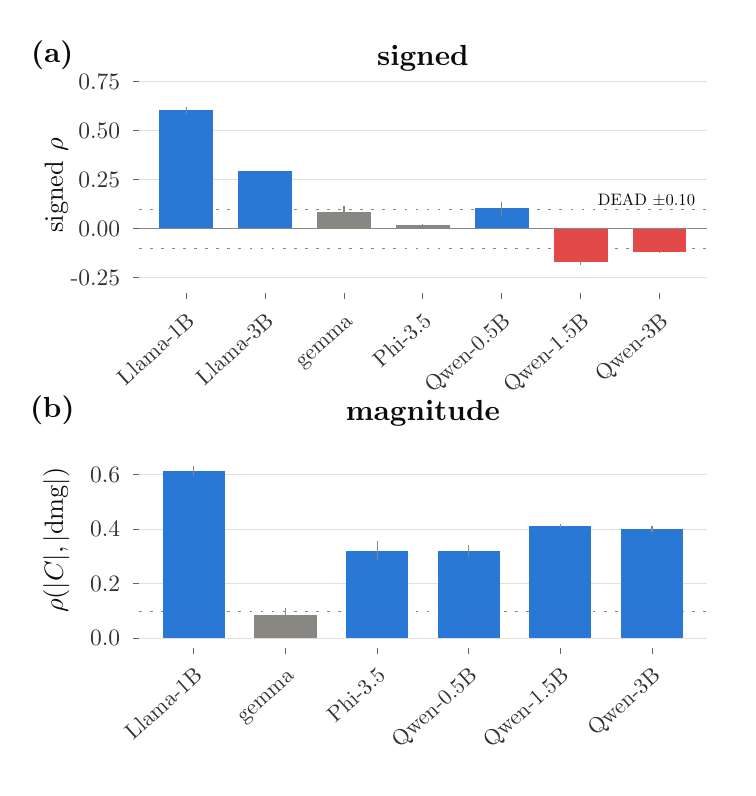
\begin{tikzpicture}[x=1pt,y=1pt]
\definecolor{fillColor}{RGB}{255,255,255}
\path[use as bounding box,fill=fillColor,fill opacity=0.00] (0,0) rectangle (252.94,267.40);
\begin{scope}
\path[clip] (  0.00,  0.00) rectangle (252.94,267.40);
\definecolor{drawColor}{RGB}{255,255,255}
\definecolor{fillColor}{RGB}{255,255,255}

\path[draw=drawColor,line width= 0.6pt,line join=round,line cap=round,fill=fillColor] (  0.00,  0.00) rectangle (252.94,267.40);
\end{scope}
\begin{scope}
\path[clip] (  5.50,133.70) rectangle (247.44,261.90);
\definecolor{fillColor}{RGB}{255,255,255}

\path[fill=fillColor] (  5.50,133.70) rectangle (247.44,261.90);
\end{scope}
\begin{scope}
\path[clip] (  5.50,  5.50) rectangle (247.44,133.70);
\definecolor{fillColor}{RGB}{255,255,255}

\path[fill=fillColor] (  5.50,  5.50) rectangle (247.44,133.70);
\end{scope}
\begin{scope}
\path[clip] ( 40.17,171.41) rectangle (245.44,249.39);
\definecolor{drawColor}{RGB}{225,224,217}

\path[draw=drawColor,line width= 0.3pt,line join=round] ( 40.17,177.08) --
	(245.44,177.08);

\path[draw=drawColor,line width= 0.3pt,line join=round] ( 40.17,194.80) --
	(245.44,194.80);

\path[draw=drawColor,line width= 0.3pt,line join=round] ( 40.17,212.53) --
	(245.44,212.53);

\path[draw=drawColor,line width= 0.3pt,line join=round] ( 40.17,230.25) --
	(245.44,230.25);

\path[draw=drawColor,line width= 0.3pt,line join=round] ( 40.17,247.97) --
	(245.44,247.97);
\definecolor{drawColor}{RGB}{137,135,129}

\path[draw=drawColor,line width= 0.3pt,dash pattern=on 1pt off 3pt ,line join=round] ( 40.17,187.71) -- (245.44,187.71);

\path[draw=drawColor,line width= 0.3pt,dash pattern=on 1pt off 3pt ,line join=round] ( 40.17,201.89) -- (245.44,201.89);
\definecolor{fillColor}{RGB}{42,120,214}

\path[fill=fillColor] ( 47.58,194.80) rectangle ( 66.97,237.47);

\path[fill=fillColor] ( 76.09,194.80) rectangle ( 95.48,215.43);
\definecolor{fillColor}{RGB}{137,135,129}

\path[fill=fillColor] (104.60,194.80) rectangle (123.99,200.77);

\path[fill=fillColor] (133.11,194.80) rectangle (152.50,196.00);
\definecolor{fillColor}{RGB}{42,120,214}

\path[fill=fillColor] (161.63,194.80) rectangle (181.01,202.11);
\definecolor{fillColor}{RGB}{227,73,72}

\path[fill=fillColor] (190.14,182.64) rectangle (209.52,194.80);

\path[fill=fillColor] (218.65,186.36) rectangle (238.03,194.80);

\path[draw=drawColor,line width= 0.3pt,line join=round] ( 40.17,194.80) -- (245.44,194.80);

\path[draw=drawColor,line width= 0.4pt,line join=round] ( 57.28,238.81) --
	( 57.28,238.81);

\path[draw=drawColor,line width= 0.4pt,line join=round] ( 57.28,238.81) --
	( 57.28,236.13);

\path[draw=drawColor,line width= 0.4pt,line join=round] ( 57.28,236.13) --
	( 57.28,236.13);

\path[draw=drawColor,line width= 0.4pt,line join=round] (114.30,202.85) --
	(114.30,202.85);

\path[draw=drawColor,line width= 0.4pt,line join=round] (114.30,202.85) --
	(114.30,198.68);

\path[draw=drawColor,line width= 0.4pt,line join=round] (114.30,198.68) --
	(114.30,198.68);

\path[draw=drawColor,line width= 0.4pt,line join=round] (142.81,196.63) --
	(142.81,196.63);

\path[draw=drawColor,line width= 0.4pt,line join=round] (142.81,196.63) --
	(142.81,195.38);

\path[draw=drawColor,line width= 0.4pt,line join=round] (142.81,195.38) --
	(142.81,195.38);

\path[draw=drawColor,line width= 0.4pt,line join=round] (171.32,204.44) --
	(171.32,204.44);

\path[draw=drawColor,line width= 0.4pt,line join=round] (171.32,204.44) --
	(171.32,199.77);

\path[draw=drawColor,line width= 0.4pt,line join=round] (171.32,199.77) --
	(171.32,199.77);

\path[draw=drawColor,line width= 0.4pt,line join=round] (199.83,183.52) --
	(199.83,183.52);

\path[draw=drawColor,line width= 0.4pt,line join=round] (199.83,183.52) --
	(199.83,181.75);

\path[draw=drawColor,line width= 0.4pt,line join=round] (199.83,181.75) --
	(199.83,181.75);

\path[draw=drawColor,line width= 0.4pt,line join=round] (228.34,186.84) --
	(228.34,186.84);

\path[draw=drawColor,line width= 0.4pt,line join=round] (228.34,186.84) --
	(228.34,185.88);

\path[draw=drawColor,line width= 0.4pt,line join=round] (228.34,185.88) --
	(228.34,185.88);
\definecolor{drawColor}{RGB}{11,11,11}

\node[text=drawColor,anchor=base east,inner sep=0pt, outer sep=0pt, scale=  0.60] at (241.17,203.14) {DEAD $\pm$0.10};
\end{scope}
\begin{scope}
\path[clip] (  0.00,  0.00) rectangle (252.94,267.40);
\definecolor{drawColor}{gray}{0.20}

\node[text=drawColor,anchor=base east,inner sep=0pt, outer sep=0pt, scale=  0.85] at ( 33.45,174.31) {-0.25};

\node[text=drawColor,anchor=base east,inner sep=0pt, outer sep=0pt, scale=  0.85] at ( 33.45,192.04) {0.00};

\node[text=drawColor,anchor=base east,inner sep=0pt, outer sep=0pt, scale=  0.85] at ( 33.45,209.76) {0.25};

\node[text=drawColor,anchor=base east,inner sep=0pt, outer sep=0pt, scale=  0.85] at ( 33.45,227.48) {0.50};

\node[text=drawColor,anchor=base east,inner sep=0pt, outer sep=0pt, scale=  0.85] at ( 33.45,245.21) {0.75};
\end{scope}
\begin{scope}
\path[clip] (  0.00,  0.00) rectangle (252.94,267.40);
\definecolor{drawColor}{gray}{0.40}

\path[draw=drawColor,line width= 0.3pt,line join=round] ( 38.17,177.08) --
	( 40.17,177.08);

\path[draw=drawColor,line width= 0.3pt,line join=round] ( 38.17,194.80) --
	( 40.17,194.80);

\path[draw=drawColor,line width= 0.3pt,line join=round] ( 38.17,212.53) --
	( 40.17,212.53);

\path[draw=drawColor,line width= 0.3pt,line join=round] ( 38.17,230.25) --
	( 40.17,230.25);

\path[draw=drawColor,line width= 0.3pt,line join=round] ( 38.17,247.97) --
	( 40.17,247.97);
\end{scope}
\begin{scope}
\path[clip] (  0.00,  0.00) rectangle (252.94,267.40);
\definecolor{drawColor}{gray}{0.40}

\path[draw=drawColor,line width= 0.3pt,line join=round] ( 57.28,169.41) --
	( 57.28,171.41);

\path[draw=drawColor,line width= 0.3pt,line join=round] ( 85.79,169.41) --
	( 85.79,171.41);

\path[draw=drawColor,line width= 0.3pt,line join=round] (114.30,169.41) --
	(114.30,171.41);

\path[draw=drawColor,line width= 0.3pt,line join=round] (142.81,169.41) --
	(142.81,171.41);

\path[draw=drawColor,line width= 0.3pt,line join=round] (171.32,169.41) --
	(171.32,171.41);

\path[draw=drawColor,line width= 0.3pt,line join=round] (199.83,169.41) --
	(199.83,171.41);

\path[draw=drawColor,line width= 0.3pt,line join=round] (228.34,169.41) --
	(228.34,171.41);
\end{scope}
\begin{scope}
\path[clip] (  0.00,  0.00) rectangle (252.94,267.40);
\definecolor{drawColor}{gray}{0.20}

\node[text=drawColor,rotate= 42.00,anchor=base east,inner sep=0pt, outer sep=0pt, scale=  0.80] at ( 60.76,160.81) {Llama-1B};

\node[text=drawColor,rotate= 42.00,anchor=base east,inner sep=0pt, outer sep=0pt, scale=  0.80] at ( 89.27,160.81) {Llama-3B};

\node[text=drawColor,rotate= 42.00,anchor=base east,inner sep=0pt, outer sep=0pt, scale=  0.80] at (117.78,160.81) {gemma};

\node[text=drawColor,rotate= 42.00,anchor=base east,inner sep=0pt, outer sep=0pt, scale=  0.80] at (146.29,160.81) {Phi-3.5};

\node[text=drawColor,rotate= 42.00,anchor=base east,inner sep=0pt, outer sep=0pt, scale=  0.80] at (174.80,160.81) {Qwen-0.5B};

\node[text=drawColor,rotate= 42.00,anchor=base east,inner sep=0pt, outer sep=0pt, scale=  0.80] at (203.31,160.81) {Qwen-1.5B};

\node[text=drawColor,rotate= 42.00,anchor=base east,inner sep=0pt, outer sep=0pt, scale=  0.80] at (231.82,160.81) {Qwen-3B};
\end{scope}
\begin{scope}
\path[clip] (  0.00,  0.00) rectangle (252.94,267.40);
\definecolor{drawColor}{RGB}{11,11,11}

\node[text=drawColor,rotate= 90.00,anchor=base,inner sep=0pt, outer sep=0pt, scale=  0.95] at ( 12.68,210.40) {signed $\rho$};
\end{scope}
\begin{scope}
\path[clip] (  0.00,  0.00) rectangle (252.94,267.40);
\definecolor{drawColor}{RGB}{11,11,11}

\node[text=drawColor,anchor=base,inner sep=0pt, outer sep=0pt, scale=  1.05] at (142.81,253.66) {\bfseries signed};
\end{scope}
\begin{scope}
\path[clip] (  0.00,  0.00) rectangle (252.94,267.40);
\definecolor{drawColor}{RGB}{11,11,11}

\node[text=drawColor,anchor=base,inner sep=0pt, outer sep=0pt, scale=  1.05] at (  8.89,254.76) {\bfseries (a)};
\end{scope}
\begin{scope}
\path[clip] ( 40.17, 43.21) rectangle (245.44,121.19);
\definecolor{drawColor}{RGB}{225,224,217}

\path[draw=drawColor,line width= 0.3pt,line join=round] ( 40.17, 46.75) --
	(245.44, 46.75);

\path[draw=drawColor,line width= 0.3pt,line join=round] ( 40.17, 66.45) --
	(245.44, 66.45);

\path[draw=drawColor,line width= 0.3pt,line join=round] ( 40.17, 86.14) --
	(245.44, 86.14);

\path[draw=drawColor,line width= 0.3pt,line join=round] ( 40.17,105.83) --
	(245.44,105.83);
\definecolor{drawColor}{RGB}{137,135,129}

\path[draw=drawColor,line width= 0.3pt,dash pattern=on 1pt off 3pt ,line join=round] ( 40.17, 56.60) -- (245.44, 56.60);
\definecolor{fillColor}{RGB}{42,120,214}

\path[fill=fillColor] ( 48.78, 46.75) rectangle ( 71.29,107.14);
\definecolor{fillColor}{RGB}{137,135,129}

\path[fill=fillColor] ( 81.89, 46.75) rectangle (104.40, 55.20);
\definecolor{fillColor}{RGB}{42,120,214}

\path[fill=fillColor] (115.00, 46.75) rectangle (137.51, 78.40);

\path[fill=fillColor] (148.11, 46.75) rectangle (170.62, 78.23);

\path[fill=fillColor] (181.21, 46.75) rectangle (203.73, 87.36);

\path[fill=fillColor] (214.32, 46.75) rectangle (236.84, 86.27);

\path[draw=drawColor,line width= 0.4pt,line join=round] ( 60.04,108.97) --
	( 60.04,108.97);

\path[draw=drawColor,line width= 0.4pt,line join=round] ( 60.04,108.97) --
	( 60.04,105.31);

\path[draw=drawColor,line width= 0.4pt,line join=round] ( 60.04,105.31) --
	( 60.04,105.31);

\path[draw=drawColor,line width= 0.4pt,line join=round] ( 93.15, 57.66) --
	( 93.15, 57.66);

\path[draw=drawColor,line width= 0.4pt,line join=round] ( 93.15, 57.66) --
	( 93.15, 52.74);

\path[draw=drawColor,line width= 0.4pt,line join=round] ( 93.15, 52.74) --
	( 93.15, 52.74);

\path[draw=drawColor,line width= 0.4pt,line join=round] (126.25, 81.86) --
	(126.25, 81.86);

\path[draw=drawColor,line width= 0.4pt,line join=round] (126.25, 81.86) --
	(126.25, 74.94);

\path[draw=drawColor,line width= 0.4pt,line join=round] (126.25, 74.94) --
	(126.25, 74.94);

\path[draw=drawColor,line width= 0.4pt,line join=round] (159.36, 80.32) --
	(159.36, 80.32);

\path[draw=drawColor,line width= 0.4pt,line join=round] (159.36, 80.32) --
	(159.36, 76.15);

\path[draw=drawColor,line width= 0.4pt,line join=round] (159.36, 76.15) --
	(159.36, 76.15);

\path[draw=drawColor,line width= 0.4pt,line join=round] (192.47, 88.21) --
	(192.47, 88.21);

\path[draw=drawColor,line width= 0.4pt,line join=round] (192.47, 88.21) --
	(192.47, 86.51);

\path[draw=drawColor,line width= 0.4pt,line join=round] (192.47, 86.51) --
	(192.47, 86.51);

\path[draw=drawColor,line width= 0.4pt,line join=round] (225.58, 87.35) --
	(225.58, 87.35);

\path[draw=drawColor,line width= 0.4pt,line join=round] (225.58, 87.35) --
	(225.58, 85.18);

\path[draw=drawColor,line width= 0.4pt,line join=round] (225.58, 85.18) --
	(225.58, 85.18);
\end{scope}
\begin{scope}
\path[clip] (  0.00,  0.00) rectangle (252.94,267.40);
\definecolor{drawColor}{gray}{0.20}

\node[text=drawColor,anchor=base east,inner sep=0pt, outer sep=0pt, scale=  0.85] at ( 33.45, 43.99) {0.0};

\node[text=drawColor,anchor=base east,inner sep=0pt, outer sep=0pt, scale=  0.85] at ( 33.45, 63.68) {0.2};

\node[text=drawColor,anchor=base east,inner sep=0pt, outer sep=0pt, scale=  0.85] at ( 33.45, 83.37) {0.4};

\node[text=drawColor,anchor=base east,inner sep=0pt, outer sep=0pt, scale=  0.85] at ( 33.45,103.07) {0.6};
\end{scope}
\begin{scope}
\path[clip] (  0.00,  0.00) rectangle (252.94,267.40);
\definecolor{drawColor}{gray}{0.40}

\path[draw=drawColor,line width= 0.3pt,line join=round] ( 38.17, 46.75) --
	( 40.17, 46.75);

\path[draw=drawColor,line width= 0.3pt,line join=round] ( 38.17, 66.45) --
	( 40.17, 66.45);

\path[draw=drawColor,line width= 0.3pt,line join=round] ( 38.17, 86.14) --
	( 40.17, 86.14);

\path[draw=drawColor,line width= 0.3pt,line join=round] ( 38.17,105.83) --
	( 40.17,105.83);
\end{scope}
\begin{scope}
\path[clip] (  0.00,  0.00) rectangle (252.94,267.40);
\definecolor{drawColor}{gray}{0.40}

\path[draw=drawColor,line width= 0.3pt,line join=round] ( 60.04, 41.21) --
	( 60.04, 43.21);

\path[draw=drawColor,line width= 0.3pt,line join=round] ( 93.15, 41.21) --
	( 93.15, 43.21);

\path[draw=drawColor,line width= 0.3pt,line join=round] (126.25, 41.21) --
	(126.25, 43.21);

\path[draw=drawColor,line width= 0.3pt,line join=round] (159.36, 41.21) --
	(159.36, 43.21);

\path[draw=drawColor,line width= 0.3pt,line join=round] (192.47, 41.21) --
	(192.47, 43.21);

\path[draw=drawColor,line width= 0.3pt,line join=round] (225.58, 41.21) --
	(225.58, 43.21);
\end{scope}
\begin{scope}
\path[clip] (  0.00,  0.00) rectangle (252.94,267.40);
\definecolor{drawColor}{gray}{0.20}

\node[text=drawColor,rotate= 42.00,anchor=base east,inner sep=0pt, outer sep=0pt, scale=  0.80] at ( 63.52, 32.61) {Llama-1B};

\node[text=drawColor,rotate= 42.00,anchor=base east,inner sep=0pt, outer sep=0pt, scale=  0.80] at ( 96.63, 32.61) {gemma};

\node[text=drawColor,rotate= 42.00,anchor=base east,inner sep=0pt, outer sep=0pt, scale=  0.80] at (129.74, 32.61) {Phi-3.5};

\node[text=drawColor,rotate= 42.00,anchor=base east,inner sep=0pt, outer sep=0pt, scale=  0.80] at (162.85, 32.61) {Qwen-0.5B};

\node[text=drawColor,rotate= 42.00,anchor=base east,inner sep=0pt, outer sep=0pt, scale=  0.80] at (195.96, 32.61) {Qwen-1.5B};

\node[text=drawColor,rotate= 42.00,anchor=base east,inner sep=0pt, outer sep=0pt, scale=  0.80] at (229.06, 32.61) {Qwen-3B};
\end{scope}
\begin{scope}
\path[clip] (  0.00,  0.00) rectangle (252.94,267.40);
\definecolor{drawColor}{RGB}{11,11,11}

\node[text=drawColor,rotate= 90.00,anchor=base,inner sep=0pt, outer sep=0pt, scale=  0.95] at ( 12.68, 82.20) {$\rho(|C|,|$dmg$|)$};
\end{scope}
\begin{scope}
\path[clip] (  0.00,  0.00) rectangle (252.94,267.40);
\definecolor{drawColor}{RGB}{11,11,11}

\node[text=drawColor,anchor=base,inner sep=0pt, outer sep=0pt, scale=  1.05] at (142.81,125.47) {\bfseries magnitude};
\end{scope}
\begin{scope}
\path[clip] (  0.00,  0.00) rectangle (252.94,267.40);
\definecolor{drawColor}{RGB}{11,11,11}

\node[text=drawColor,anchor=base,inner sep=0pt, outer sep=0pt, scale=  1.05] at (  8.89,126.56) {\bfseries (b)};
\end{scope}
\end{tikzpicture}

\caption{Architecture-family generalization of the geometry law (companion
to Figure~\ref{fig:layerlaw}, Section~\ref{sec:regime}; discussed in the
architecture arm of Section~\ref{sec:dissociation}). \textbf{(a)} the
\emph{signed} law is Llama-specific: null on gemma/Phi (grey, $|\rho|$ below
the $0.10$ DEAD floor), inverted on Qwen. \textbf{(b)} the \emph{magnitude}
law $|C|\!\to\!|$dmg$|$ transfers on four of five non-Llama families; gemma
is the sole failure (grey, below the $0.10$ DEAD floor). Error bars are
3-seed s.d.\ where seeds exist.}
\label{fig:crossarch}
\end{figure}


\subsection{The editability band across architectures}
The layer law above is stated over the depth range in which an edit
\emph{takes} at all. That range is itself architecture-dependent, and its
shape bounds where any geometry-to-damage law can even be measured.
Figure~\ref{fig:band} traces the single-edit success rate against
\emph{relative} depth --- edited layer index divided by the model's layer
count --- for real single-fact edits across six models spanning four
architecture families (1B--20B parameters).

Two qualitatively different band shapes appear. The Llama and
Pythia~\citep{biderman2023pythia} models
hold a \emph{wide plateau}: Llama-8B keeps edit success at or above
\llamaEightEsrMin{} at every tested depth (one to three seeds per depth), and
both Pythia sizes stay healthy through \pythiaHealthyDepth{} relative depth
(Pythia-1.4B $\geq\pythiaOneFourEsrMin{}$, Pythia-2.8B
$\geq\pythiaTwoEightEsrMin{}$; 3 seeds each). GPT-J-6B~\citep{wang2021gptj}
instead shows a
\emph{gradual decay}: success falls from \gptjEsrA{}/\gptjEsrB{} in the lower
half of the network to \gptjEsrC{} at three-quarter depth and \gptjEsrD{} at
seven-eighths depth (3 seeds). GPT-NeoX-20B~\citep{black2022neox} shows the
sharpest form, a
\emph{shallow-band cliff}: edit success is \neoxEsrShallow{} at roughly
one-quarter depth, already \neoxEsrMid{} by one-third depth, and collapses to
\neoxEsrHalf{} at half-depth (3 seeds), so at 20B the reliably editable band is
confined to the earliest layers.

Where GPT-NeoX-20B remains editable, the geometry-to-damage coupling is weak.
Its within-probe key-cosine coupling stays below the $0.10$ level we treat as
null throughout the paper (the DEAD floor marked in
Figures~\ref{fig:layerlaw}--\ref{fig:crossarch}) across the band
($\rho_C\leq\neoxRhoCmax{}$), and the closed-form
\SxC{} coupling rises with depth only to
\neoxRhoSCa{}/\neoxRhoSCb{}/\neoxRhoSCc{} at its L11/L16/L22 band. This mirrors
the attenuation already seen within the Llama family at 8B: the closed-form law
that is sharp at $\leq$3B weakens at the largest scales we test, whether
measured within one family or across a distinct 20B architecture. The Pythia
family sharpens this into a dissociation: although its editable band is the
widest outside Llama, the geometry coupling is null at every probed layer of
both sizes
% PYTHIA_mechanism_sc_table.json max |within_probe_rho_C| = |-0.0941| (pythia28b L8); max |within_probe_rho_SC| = |-0.0778| (pythia28b L8); groups pythia14b L6/L12/L15 + pythia28b L8/L16/L20, 3-seed pooled, mean damage negative (net-improvement regime)
($|\rho_C|\leq\pythiaRhoCabsMax{}$, $|\rho_{SC}|\leq\pythiaRhoSCabsMax{}$;
3 seeds, net-improvement regime), so a wide editable band does not imply
geometry-carried damage. In the cross-architecture taxonomy of
Section~\ref{sec:dissociation}, Pythia joins gemma and Phi in the null camp
rather than Qwen's inversion.

% =====================================================================
% fig:band — editability band across architectures (single-edit success
% rate vs relative edit depth, one line per model). Body ported from the
% R/tikzDevice pipeline (figures/figG.tex, IEEE single-column dimensions);
% no new numbers. Five series read from esr_band_table.json (cf-dataset
% rows); the GPT-NeoX-20B series reads esr from NEOX20B_law_table.json
% (3-seed mean per layer) placed on the relative-depth axis via layer/44
% (44 = GPT-NeoX-20B transformer-layer count, public HF-config constant).
% Presented in Section~\ref{sec:regime}.
% Regenerate: Rscript figures/make_figures_ieee.R
% esr_band_table.json::curves['gptj|rome|cf']['0.8571'].mean_esr = 0.4017
% NEOX20B_law_table.json::rows[layer=22].esr (3-seed mean) = 0.50 at depth 22/44=0.5
% =====================================================================
\begin{figure}[t]
\centering
% =====================================================================
% figG  — R/ggplot2 -> tikzDevice (parallel to ../figures-tex/figG_band.tex)
% Canonical-JSON-only. Regenerate: Rscript figures/make_figures_ieee.R
% Provenance (JSON path :: field = plotted value), one line per series:
% SOURCE: results/esr_band_table.json :: curves['gptj|rome|cf']['0.5'].mean_esr = 0.9933
% SOURCE: results/esr_band_table.json :: curves['gptj|rome|cf']['0.6429'].mean_esr = 0.9833
% SOURCE: results/esr_band_table.json :: curves['gptj|rome|cf']['0.75'].mean_esr = 0.7850
% SOURCE: results/esr_band_table.json :: curves['gptj|rome|cf']['0.8571'].mean_esr = 0.4017
% SOURCE: results/esr_band_table.json :: curves['llama1b|rome|cf']['0.75'].mean_esr = 0.9950
% SOURCE: results/esr_band_table.json :: curves['llama8b|rome|cf']['0.5'].mean_esr = 1.0000
% SOURCE: results/esr_band_table.json :: curves['llama8b|rome|cf']['0.75'].mean_esr = 0.9983
% SOURCE: results/esr_band_table.json :: curves['llama8b|rome|cf']['0.875'].mean_esr = 1.0000
% SOURCE: results/esr_band_table.json :: curves['pythia14b|rome|cf']['0.25'].mean_esr = 0.9983
% SOURCE: results/esr_band_table.json :: curves['pythia14b|rome|cf']['0.5'].mean_esr = 0.9967
% SOURCE: results/esr_band_table.json :: curves['pythia14b|rome|cf']['0.625'].mean_esr = 0.9967
% SOURCE: results/esr_band_table.json :: curves['pythia28b|rome|cf']['0.25'].mean_esr = 0.9983
% SOURCE: results/esr_band_table.json :: curves['pythia28b|rome|cf']['0.5'].mean_esr = 0.9967
% SOURCE: results/esr_band_table.json :: curves['pythia28b|rome|cf']['0.625'].mean_esr = 0.9417
% SOURCE: results/NEOX20B_law_table.json :: rows[layer=11].esr (3-seed mean); depth_frac = 11/44 (public config value) = 0.9733
% SOURCE: results/NEOX20B_law_table.json :: rows[layer=16].esr (3-seed mean); depth_frac = 16/44 (public config value) = 0.8833
% SOURCE: results/NEOX20B_law_table.json :: rows[layer=22].esr (3-seed mean); depth_frac = 22/44 (public config value) = 0.5000
% =====================================================================
% !TEX encoding = UTF-8 Unicode
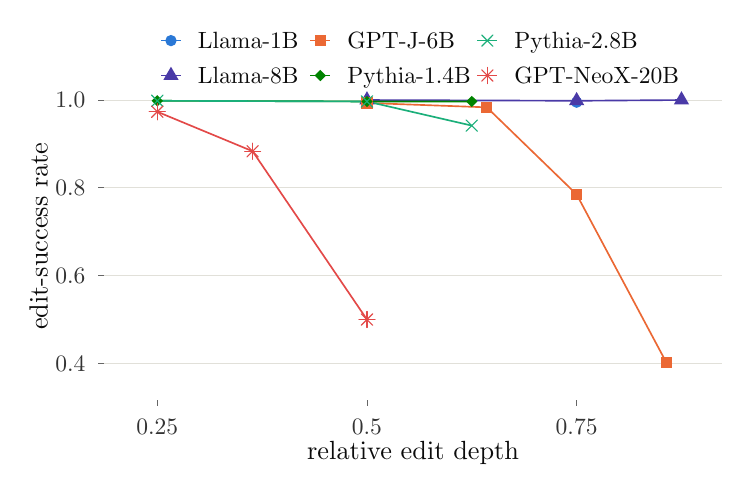
\begin{tikzpicture}[x=1pt,y=1pt]
\definecolor{fillColor}{RGB}{255,255,255}
\path[use as bounding box,fill=fillColor,fill opacity=0.00] (0,0) rectangle (252.94,158.99);
\begin{scope}
\path[clip] (  0.00,  0.00) rectangle (252.94,158.99);
\definecolor{fillColor}{RGB}{255,255,255}

\path[fill=fillColor] (  0.00, -0.00) rectangle (252.94,158.99);
\end{scope}
\begin{scope}
\path[clip] ( 27.59, 24.34) rectangle (250.95,143.00);
\definecolor{drawColor}{RGB}{225,224,217}

\path[draw=drawColor,line width= 0.3pt,line join=round] ( 27.59, 37.66) --
	(250.95, 37.66);

\path[draw=drawColor,line width= 0.3pt,line join=round] ( 27.59, 69.39) --
	(250.95, 69.39);

\path[draw=drawColor,line width= 0.3pt,line join=round] ( 27.59,101.12) --
	(250.95,101.12);

\path[draw=drawColor,line width= 0.3pt,line join=round] ( 27.59,132.84) --
	(250.95,132.84);
\definecolor{drawColor}{RGB}{74,58,167}

\path[draw=drawColor,line width= 0.6pt,line join=round] (122.60,132.84) --
	(198.36,132.57) --
	(236.25,132.84);
\definecolor{drawColor}{RGB}{235,104,52}

\path[draw=drawColor,line width= 0.6pt,line join=round] (122.60,131.78) --
	(165.91,130.20) --
	(198.36, 98.74) --
	(230.82, 37.93);
\definecolor{drawColor}{RGB}{0,131,0}

\path[draw=drawColor,line width= 0.6pt,line join=round] ( 46.84,132.57) --
	(122.60,132.32) --
	(160.48,132.32);
\definecolor{drawColor}{RGB}{27,175,122}

\path[draw=drawColor,line width= 0.6pt,line join=round] ( 46.84,132.57) --
	(122.60,132.32) --
	(160.48,123.60);
\definecolor{drawColor}{RGB}{227,73,72}

\path[draw=drawColor,line width= 0.6pt,line join=round] ( 46.84,128.61) --
	( 81.27,114.34) --
	(122.60, 53.53);
\definecolor{fillColor}{RGB}{42,120,214}

\path[fill=fillColor] (198.36,132.05) circle (  2.05);
\definecolor{fillColor}{RGB}{74,58,167}

\path[fill=fillColor] (122.60,136.04) --
	(125.36,131.25) --
	(119.83,131.25) --
	cycle;

\path[fill=fillColor] (198.36,135.77) --
	(201.13,130.98) --
	(195.60,130.98) --
	cycle;

\path[fill=fillColor] (236.25,136.04) --
	(239.01,131.25) --
	(233.48,131.25) --
	cycle;
\definecolor{fillColor}{RGB}{235,104,52}

\path[fill=fillColor] (120.55,129.73) --
	(124.65,129.73) --
	(124.65,133.83) --
	(120.55,133.83) --
	cycle;

\path[fill=fillColor] (163.85,128.14) --
	(167.96,128.14) --
	(167.96,132.25) --
	(163.85,132.25) --
	cycle;

\path[fill=fillColor] (196.31, 96.69) --
	(200.42, 96.69) --
	(200.42,100.79) --
	(196.31,100.79) --
	cycle;

\path[fill=fillColor] (228.77, 35.88) --
	(232.87, 35.88) --
	(232.87, 39.99) --
	(228.77, 39.99) --
	cycle;
\definecolor{fillColor}{RGB}{0,131,0}

\path[fill=fillColor] ( 44.78,132.57) --
	( 46.84,134.63) --
	( 48.89,132.57) --
	( 46.84,130.52) --
	cycle;

\path[fill=fillColor] (120.55,132.32) --
	(122.60,134.37) --
	(124.65,132.32) --
	(122.60,130.27) --
	cycle;

\path[fill=fillColor] (158.43,132.32) --
	(160.48,134.37) --
	(162.54,132.32) --
	(160.48,130.27) --
	cycle;
\definecolor{drawColor}{RGB}{27,175,122}

\path[draw=drawColor,line width= 0.4pt,line join=round,line cap=round] ( 44.78,130.52) -- ( 48.89,134.63);

\path[draw=drawColor,line width= 0.4pt,line join=round,line cap=round] ( 44.78,134.63) -- ( 48.89,130.52);

\path[draw=drawColor,line width= 0.4pt,line join=round,line cap=round] (120.55,130.27) -- (124.65,134.37);

\path[draw=drawColor,line width= 0.4pt,line join=round,line cap=round] (120.55,134.37) -- (124.65,130.27);

\path[draw=drawColor,line width= 0.4pt,line join=round,line cap=round] (158.43,121.54) -- (162.54,125.65);

\path[draw=drawColor,line width= 0.4pt,line join=round,line cap=round] (158.43,125.65) -- (162.54,121.54);
\definecolor{drawColor}{RGB}{227,73,72}

\path[draw=drawColor,line width= 0.4pt,line join=round,line cap=round] ( 44.78,126.56) -- ( 48.89,130.67);

\path[draw=drawColor,line width= 0.4pt,line join=round,line cap=round] ( 44.78,130.67) -- ( 48.89,126.56);

\path[draw=drawColor,line width= 0.4pt,line join=round,line cap=round] ( 43.93,128.61) -- ( 49.74,128.61);

\path[draw=drawColor,line width= 0.4pt,line join=round,line cap=round] ( 46.84,125.71) -- ( 46.84,131.52);

\path[draw=drawColor,line width= 0.4pt,line join=round,line cap=round] ( 79.22,112.28) -- ( 83.33,116.39);

\path[draw=drawColor,line width= 0.4pt,line join=round,line cap=round] ( 79.22,116.39) -- ( 83.33,112.28);

\path[draw=drawColor,line width= 0.4pt,line join=round,line cap=round] ( 78.37,114.34) -- ( 84.18,114.34);

\path[draw=drawColor,line width= 0.4pt,line join=round,line cap=round] ( 81.27,111.43) -- ( 81.27,117.24);

\path[draw=drawColor,line width= 0.4pt,line join=round,line cap=round] (120.55, 51.47) -- (124.65, 55.58);

\path[draw=drawColor,line width= 0.4pt,line join=round,line cap=round] (120.55, 55.58) -- (124.65, 51.47);

\path[draw=drawColor,line width= 0.4pt,line join=round,line cap=round] (119.70, 53.53) -- (125.50, 53.53);

\path[draw=drawColor,line width= 0.4pt,line join=round,line cap=round] (122.60, 50.62) -- (122.60, 56.43);
\end{scope}
\begin{scope}
\path[clip] (  0.00,  0.00) rectangle (252.94,158.99);
\definecolor{drawColor}{gray}{0.20}

\node[text=drawColor,anchor=base east,inner sep=0pt, outer sep=0pt, scale=  0.85] at ( 20.87, 34.90) {0.4};

\node[text=drawColor,anchor=base east,inner sep=0pt, outer sep=0pt, scale=  0.85] at ( 20.87, 66.62) {0.6};

\node[text=drawColor,anchor=base east,inner sep=0pt, outer sep=0pt, scale=  0.85] at ( 20.87, 98.35) {0.8};

\node[text=drawColor,anchor=base east,inner sep=0pt, outer sep=0pt, scale=  0.85] at ( 20.87,130.08) {1.0};
\end{scope}
\begin{scope}
\path[clip] (  0.00,  0.00) rectangle (252.94,158.99);
\definecolor{drawColor}{gray}{0.40}

\path[draw=drawColor,line width= 0.3pt,line join=round] ( 25.59, 37.66) --
	( 27.59, 37.66);

\path[draw=drawColor,line width= 0.3pt,line join=round] ( 25.59, 69.39) --
	( 27.59, 69.39);

\path[draw=drawColor,line width= 0.3pt,line join=round] ( 25.59,101.12) --
	( 27.59,101.12);

\path[draw=drawColor,line width= 0.3pt,line join=round] ( 25.59,132.84) --
	( 27.59,132.84);
\end{scope}
\begin{scope}
\path[clip] (  0.00,  0.00) rectangle (252.94,158.99);
\definecolor{drawColor}{gray}{0.40}

\path[draw=drawColor,line width= 0.3pt,line join=round] ( 46.84, 22.34) --
	( 46.84, 24.34);

\path[draw=drawColor,line width= 0.3pt,line join=round] (122.60, 22.34) --
	(122.60, 24.34);

\path[draw=drawColor,line width= 0.3pt,line join=round] (198.36, 22.34) --
	(198.36, 24.34);
\end{scope}
\begin{scope}
\path[clip] (  0.00,  0.00) rectangle (252.94,158.99);
\definecolor{drawColor}{gray}{0.20}

\node[text=drawColor,anchor=base,inner sep=0pt, outer sep=0pt, scale=  0.85] at ( 46.84, 12.08) {0.25};

\node[text=drawColor,anchor=base,inner sep=0pt, outer sep=0pt, scale=  0.85] at (122.60, 12.08) {0.5};

\node[text=drawColor,anchor=base,inner sep=0pt, outer sep=0pt, scale=  0.85] at (198.36, 12.08) {0.75};
\end{scope}
\begin{scope}
\path[clip] (  0.00,  0.00) rectangle (252.94,158.99);
\definecolor{drawColor}{RGB}{11,11,11}

\node[text=drawColor,anchor=base,inner sep=0pt, outer sep=0pt, scale=  0.95] at (139.27,  3.06) {relative edit depth};
\end{scope}
\begin{scope}
\path[clip] (  0.00,  0.00) rectangle (252.94,158.99);
\definecolor{drawColor}{RGB}{11,11,11}

\node[text=drawColor,rotate= 90.00,anchor=base,inner sep=0pt, outer sep=0pt, scale=  0.95] at (  7.18, 83.67) {edit-success rate};
\end{scope}
\begin{scope}
\path[clip] (  0.00,  0.00) rectangle (252.94,158.99);
\definecolor{drawColor}{RGB}{42,120,214}

\path[draw=drawColor,line width= 0.6pt,line join=round] ( 48.18,154.31) -- ( 55.38,154.31);
\definecolor{fillColor}{RGB}{42,120,214}

\path[fill=fillColor] ( 51.78,154.31) circle (  2.05);
\end{scope}
\begin{scope}
\path[clip] (  0.00,  0.00) rectangle (252.94,158.99);
\definecolor{drawColor}{RGB}{74,58,167}

\path[draw=drawColor,line width= 0.6pt,line join=round] ( 48.18,141.68) -- ( 55.38,141.68);
\definecolor{fillColor}{RGB}{74,58,167}

\path[fill=fillColor] ( 51.78,144.88) --
	( 54.55,140.09) --
	( 49.02,140.09) --
	cycle;
\end{scope}
\begin{scope}
\path[clip] (  0.00,  0.00) rectangle (252.94,158.99);
\definecolor{drawColor}{RGB}{235,104,52}

\path[draw=drawColor,line width= 0.6pt,line join=round] (102.15,154.31) -- (109.35,154.31);
\definecolor{fillColor}{RGB}{235,104,52}

\path[fill=fillColor] (103.70,152.25) --
	(107.80,152.25) --
	(107.80,156.36) --
	(103.70,156.36) --
	cycle;
\end{scope}
\begin{scope}
\path[clip] (  0.00,  0.00) rectangle (252.94,158.99);
\definecolor{drawColor}{RGB}{0,131,0}

\path[draw=drawColor,line width= 0.6pt,line join=round] (102.15,141.68) -- (109.35,141.68);
\definecolor{fillColor}{RGB}{0,131,0}

\path[fill=fillColor] (103.70,141.68) --
	(105.75,143.74) --
	(107.80,141.68) --
	(105.75,139.63) --
	cycle;
\end{scope}
\begin{scope}
\path[clip] (  0.00,  0.00) rectangle (252.94,158.99);
\definecolor{drawColor}{RGB}{27,175,122}

\path[draw=drawColor,line width= 0.6pt,line join=round] (162.50,154.31) -- (169.70,154.31);

\path[draw=drawColor,line width= 0.4pt,line join=round,line cap=round] (164.05,152.25) -- (168.15,156.36);

\path[draw=drawColor,line width= 0.4pt,line join=round,line cap=round] (164.05,156.36) -- (168.15,152.25);
\end{scope}
\begin{scope}
\path[clip] (  0.00,  0.00) rectangle (252.94,158.99);
\definecolor{drawColor}{RGB}{227,73,72}

\path[draw=drawColor,line width= 0.6pt,line join=round] (162.50,141.68) -- (169.70,141.68);

\path[draw=drawColor,line width= 0.4pt,line join=round,line cap=round] (164.05,139.63) -- (168.15,143.74);

\path[draw=drawColor,line width= 0.4pt,line join=round,line cap=round] (164.05,143.74) -- (168.15,139.63);

\path[draw=drawColor,line width= 0.4pt,line join=round,line cap=round] (163.20,141.68) -- (169.00,141.68);

\path[draw=drawColor,line width= 0.4pt,line join=round,line cap=round] (166.10,138.78) -- (166.10,144.59);
\end{scope}
\begin{scope}
\path[clip] (  0.00,  0.00) rectangle (252.94,158.99);
\definecolor{drawColor}{RGB}{11,11,11}

\node[text=drawColor,anchor=base west,inner sep=0pt, outer sep=0pt, scale=  0.85] at ( 61.53,151.54) {Llama-1B};
\end{scope}
\begin{scope}
\path[clip] (  0.00,  0.00) rectangle (252.94,158.99);
\definecolor{drawColor}{RGB}{11,11,11}

\node[text=drawColor,anchor=base west,inner sep=0pt, outer sep=0pt, scale=  0.85] at ( 61.53,138.92) {Llama-8B};
\end{scope}
\begin{scope}
\path[clip] (  0.00,  0.00) rectangle (252.94,158.99);
\definecolor{drawColor}{RGB}{11,11,11}

\node[text=drawColor,anchor=base west,inner sep=0pt, outer sep=0pt, scale=  0.85] at (115.50,151.54) {GPT-J-6B};
\end{scope}
\begin{scope}
\path[clip] (  0.00,  0.00) rectangle (252.94,158.99);
\definecolor{drawColor}{RGB}{11,11,11}

\node[text=drawColor,anchor=base west,inner sep=0pt, outer sep=0pt, scale=  0.85] at (115.50,138.92) {Pythia-1.4B};
\end{scope}
\begin{scope}
\path[clip] (  0.00,  0.00) rectangle (252.94,158.99);
\definecolor{drawColor}{RGB}{11,11,11}

\node[text=drawColor,anchor=base west,inner sep=0pt, outer sep=0pt, scale=  0.85] at (175.85,151.54) {Pythia-2.8B};
\end{scope}
\begin{scope}
\path[clip] (  0.00,  0.00) rectangle (252.94,158.99);
\definecolor{drawColor}{RGB}{11,11,11}

\node[text=drawColor,anchor=base west,inner sep=0pt, outer sep=0pt, scale=  0.85] at (175.85,138.92) {GPT-NeoX-20B};
\end{scope}
\end{tikzpicture}

\caption{Single-edit success rate versus relative edit depth (edited layer
index divided by the number of layers) for single-fact edits across six models
spanning four architecture families (1B--20B parameters). The reliably editable
depth band is architecture-dependent: the Llama and Pythia models sustain
near-perfect edit success across the tested depths; GPT-J-6B decays gradually
with depth, succeeding on only about $0.40$ of edits by seven-eighths depth;
and GPT-NeoX-20B falls off a cliff, dropping from near-ceiling in its lowest
quarter to roughly half-success by mid-depth, so at 20B the reliably editable
band is confined to the earliest layers. Points are means over the available
seeds (up to three).}
\label{fig:band}
\end{figure}


The depth and regime results above are, by construction, purely
observational: they describe how a correlational statistic moves with depth
and scale. Section~\ref{sec:causal} closes this gap with an intervention
that manipulates the geometry directly and asks whether the damage it
predicts is also damage it causes.
